% chapter 1
\cleardoublepage
\phantomsection
\chapter{Literature Review}
\section{What, how and why parallel?}
To begin my literature review, I shall ask the broadest of questions in this specific subject field: what is parallel computing, how is it done at a fundamental level and why should it be done? While searching for the answers to these questions, I have discovered a book titled ‘Introduction to Parallel Computing’ by Ananth Grama et. al. \cite{grama_et_al_2003}

Within this book, I have found that parallel computing has been around for a while but its methods and purposes have changed over time. Grama et al. argues that parallel programming took a while to take off due to the uncertainty of hardware evolution going forward and the lack of consistent platforms to develop on. As of the book's publication this was changing however, with the standardisation of parallel platforms bringing about a much shorter development time for such projects.

The book also discusses the arguments for parallelism, as well as its real-world applications. When discussing the arguments for parallelism, the book authors suggest that pooling resources such as CPU time, memory and data links typically results in a high-performance computer, with the added benefits of high-availability, larger caching and higher aggregate bandwidth.

These benefits lend themselves well to several applications, ranging from engineering and scientific research to commercial applications such as web hosting and digital banking. One particular example that has piqued my interest is its applications in computer systems. Problems that were traditionally very computationally expensive (i.e. cryptography or distributed algorithm solving) can now be done on clusters in a much-reduced time.

Within Chapters 6 and 7 of this book, the authors expose two very different yet also very powerful methods of parallel programming. Chapter 6 covers programming using the message-passing model, a general term used to express any form of parallel program that sends its instructions to separate processes (either internally within a computer or externally to multiple nodes in a networked cluster), while Chapter 7 covers shared address space programming, which is typically achieved using POSIX threads.

Having read through both chapters, I have decided that the method best suited to my problem (i.e. building a Beowulf computer) will be message-passing. Message-passing is the older, more researched method of inter-computer parallelism with more available papers and better suited my needs as a whole for this particular project.

\section{A look into message-passing parallelism: MPI}
In order to better understand exactly why message-passing was used more often in inter-computer parallelism over shared address space parallelism, I have decided to look into methods of message-passing programming. While I have found many books on the subject matter, by far the most reputable and comprehensive title was ‘Using MPI - Portable parallel programming with the Message-Passing Interface’ by William Gropp et. al. \cite{gropp_et_al_2014}

Gropp et al. define message-passing as a collection of processes that only have local memory but maintain the ability to pass information between each other using some form of intercommunication protocol. Message-passing from once process to another inherently requires actions to be taken by both processes, which raises an interesting aside in my mind: does that mean each process within a message-passing cluster is a client/server in and of itself?

\begin{figure}[H]
    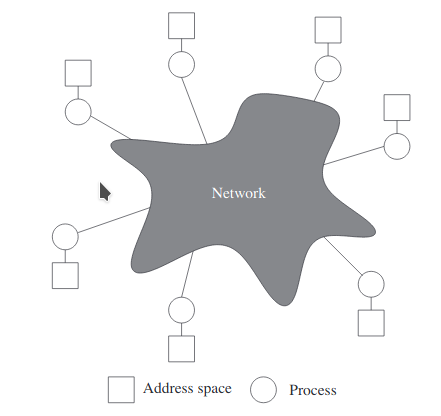
\includegraphics[width=\linewidth]{CITY3111/bitmaps/figure_1.png}
    \caption{Diagram from book showing abstract message-passing architecture\cite{gropp_et_al_2014}}
    \label{figure_1}
\end{figure}

Also expressed in this chapter is the advantages found in using a message-passing model. For one, it is incredibly versatile, allowing for easy development, debugging and deployment on a wide range of hardware. Once aside that did occur to me, which I shall address later in this section, is: how does heterogeneous hardware affect the performance of a cluster?

The main point raised in this particular chapter, however, is the performance gains to be had from utilising message-passing, which is exactly what I am hunting for in my research. According to the authors, message-passing permits the host hardware full management over its caching, thus affording the CPU full and unhindered functionality which in turn drives performance gains over even the most generously designed of single-processor machines with regards to available cache memory.

Section 1,5 and Chapter 2 of this book specifically offers insight into one particular implementation of a message-passing standard: Message-Passing Interface (MPI) and its governing body, the MPI forum. The book authors tell of the development of the MPI standard as a necessity of the time in an age where message-passing softwares were plentiful, typically too bespoke for general purpose high-performance computing (HPC) and commercial in nature. The MPI Forum concluded in 1992 they would develop a standard which was portable, open and aimed to be completed in a year. The subsequent product was MPI-1 (1994) \cite{mpi_1994}, released after little over a year of frantic development.

The MPI standard has since been revised numerous times, with its latest publication coming in 2015 \cite{mpi_2015}. MPI can therefore be relied on as a fresh and well-maintained standard based around a paradigm that is suitable for my research topic. Alas, no manner of searching I conduct can find an equivalent to compare MPI against that is as comprehensive, portable and recent as MPI appears to be. The next piece of secondary research that therefore comes to mind centres around discovering a suitable network implementation to run MPI atop.

Referring lastly back to a question I posed earlier in this section as an aside -- ``how does heterogeneous hardware affect the performance of a cluster?'', Section 7,4 of this particular book expresses how MPI manages the translation of data representation between systems with incompatible data formats. While this is encouraging news for heterogeneous clusters, it does not satisfy my curiosity and additional research will be needed to cover this topic point.

\section{Networking with MPI: TCP, InfiniBand and Open MPI}
Discovering MPI will facilitate inter-nodal computation was only the first step in assessing how I can implement my project. The next step is to try and ascertain what communication standard I can use to enable optimal link speeds between all of my nodes.

I began by searching in general terms for MPI network implementations before resolving to nuance my searches down to specific network protocols I have knowledge of, the first and most popular being the Transmission Control Protocol (TCP).

The conclusion of this research turned up two papers of interest, the first of which being `Open MPI: A Flexible High Performance MPI' by Richard L. Graham (et. al. 2005) \cite{graham_et_al_2006}. Within the abstract of this paper, Graham et. al. observe how, while the MPI Form defines a standard, MPI implementations are not cross compatible. This historically caused a swathe of specialised MPI implementations that a researcher would need to choose based on their usecase and stick to for the duration of a project.

Open MPI aims to solve some of these issues by offering the ability to include third-party software add-ons in the MPI run-time, as well as by offering novel features not available in other MPI implementations. While my usage of MPI will likely not require any of these novel features or the inclusion of third-party software during run-time, it is nonetheless an implementation worth looking into for my project.

The main interest of this paper for me can be seen in Table 1 and Table 2, however. Here, I can see the authors have conducted a test with a view to ascertain which protocol is fastest by testing the system latency in a point-to-point zero-byte ping. Unbeknown to me, TCP actually performed poorly in comparison to both the InfiniBand implementations and the Myrinet stack. While some of this may be attributed to the hardware discrepancies seen in Table 1, these figures definitely merit my further research into InfiniBand technology with Open MPI.

I performed some additional research into Open MPI \cite{shipman_et_al_2006} and discovered the InfiniBand is also very well-suited to HPC not only because of its lower latency compared to TCP but also thanks to its impressive scalability metrics. This is, however, where I had to leave my research regarding InfiniBand as the hardware costs are astronomical and greatly exceed my budget for this project.

I therefore resolved to press on with Open MPI using TCP. My next natural step was to find some programs that had been written for an Open MPI environment.

\section{Understanding Parallel Programming using Open MPI: Example software}
To garner an understanding of how Open MPI works in a practical setting, I want to find some example source code. Open MPI has an up-to-date API reference \cite{open_mpi_2020} and features workshop sessions, explaining through digital lectures how to program a basic `hello world' system. The discovered example program can be found in Appendix α.

Anyone familiar with C/C++ should understand the syntax involved in the aforementioned code snippet, the only difference is the methods in use (specifically, the four MPI methods). Referencing the Open MPI documentation, each of these methods should roughly achieve the following:

\begin{itemize}
    \item \textbf{\emph{MPI\_Init}} -- This method initialises the MPI environment either using the C/C++ arcg/argv[] pointers or with NULL values.
    \item \textbf{\emph{MPI\_Comm\_rank}} -- This method will acquire the current processes rank in the MPI `world' (i.e. the cluster). This can be useful for a number of reasons, including message-passing identification or debug printing.
    \item \textbf{\emph{MPI\_Comm\_size}} -- This method will acquire the current MPI `world' size. This is useful in ascertaining if all nodes are connecting well, as well as for dynamic task division.
    \item \textbf{\emph{MPI\_Finalize}} -- This method will clean up the MPI subroutine when called, and is typically used just before the parent function is returned.
\end{itemize}

If my understanding the API is precise, the example code will, when compiled, display a list of all ranked processes within the MPI `world' and output a `hello world' from each. To ensure my understanding is correct, I'll now attempt to display the `hello world' program in action by compiling it using the custom `mpicc' compiler also mentioned in the documentation (based upon the GNU C/C++ compiler).

\begin{figure}[H]
    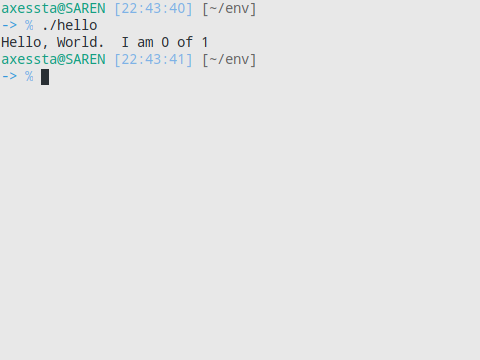
\includegraphics[width=\linewidth]{CITY3111/bitmaps/figure_2.png}
    \caption{A compiled and running copy of Barrett et. al's `hello world' program \cite{barrett_et_al_2006}}
    \label{figure_2}
\end{figure}

The Open MPI example code functions as intended and displays a `hello world' prompt, but the world only encompasses a single process at this time. In order to introduce more processes into the world, I need to introduce a runtime component which will facilitate the spawning of additional processes as well as their communication across my cluster -- even between nodes. This runtime is included in the Open MPI distribution, which I will further research in my system analysis.

\section{Discussion on an alternative to Open MPI: PVM}
In my literature review so far, I have looked at different methods available to me for creating a parallel cluster and have narrowed down on one particular framework. Before I conclude my literature review, I am going to discuss another framework that could be used and why I won't be using it.

The first, and oldest of the two frameworks is parallel virtual machine (PVM). According to its manual \cite{geist_et_al_1995}, PVM aims to provide much of the same message-passing functionality as MPI does but instead of offering each node up as individuals to solve a whole, it attempts to simulate one large, singular virtual machine upon which many processor cores co-exist.

These design difference are born out of the differences in their development and purpose, according to Dr. Elts \cite{elts_2004}. Take the development argument, for example. As we've previously discussed, MPI had a rather rapid development with a large number of stakeholders whom all had to be satiated. PVM was developed and designed earlier than MPI and by a single research group in Oak Ridge, TN with a view to create a virtual machine that could span multiple machines. MPI, in contrast, explicitly specified against parallel virtualisation within its core specification.

These differences in development and goal lead to two very different frameworks and implementations. MPI allows for flexible allocation of processes, with many topologies being feasible (likely a requirement of so many stakeholders) while PVM only allows for a master/slave architecture with poor fault tolerance if the master node falls over. Additionally, as PVM attempts to pool all memory under one virtual machine, the aforementioned cache control speedups MPI typically experiences are lost in PVM.
\vfill\break

To better explain the previous point, imagine a suitable Republic such as the French Republic. There are two main institutions at play, somewhat analogous to PVM and MPI in function. In the French Republic, the \emph{président} or \emph{présidente} appoints his or her \emph{gouvernement} who will then liaise on a regular basis, but the président retains authority in the cabinet (i.e. a master/slave architecture). This relationship can be seen as the relationship nodes are under with PVM, one of rigidity and structure.

The second pillar of any good republic's structure is the \emph{parliament}, specifically the \emph{Assemblée Nationale} in our example. The Assemblée Nationale is brought together collectively to perform a function in unison, with little to no guidance aside from a schedule (i.e. a mesh topology). This is more analogous to MPI, whose processes are loosely directed by a runtime but are otherwise free to communicate with any other member of the cluster as it sees fit.

For my purposes and function, having the flexibility of being able to choose my topology is critical. I don't yet know what programming challenges I may encounter, and having a more up-to-date and powerful tool-set seems like the best choice for my project going forward.

\section{Conclusion on Literature Review}
Within my literature review, I have investigated different methods one can utilise in order to produce a working parallel computer using commodity, open-source software and have investigated the principles underlying parallelism and why one might choose to use such methods. 

I have taken an in-depth look at the MPI standard and expressed why this standard is suitable for my project goal, and have picked out Open MPI and a popular example implementation of the MPI standard to further express its function and usefulness to my project, offering example code for reference.

I have then taken a step back from Open MPI and looked at PVM as an alternative technology with which similar projects have been completed using before, discussing the fundamental differences between them and why PVM would not be as suitable for my task as MPI.

In conclusion to my literature review, I offer an impact case study from the Research Excellence Framework of 2014 \cite{trew_et_al_2014}. Dr Trew et al. posit that the impact of MPI is far-reaching, with MPI being regarded the \emph{de-facto} standard in parallel computer programming.

This has been attributed to its wide availability, with some distribution being available for almost all architectures ranging from desktop computers to the TOP500 supercomputers (2014), and the portability associated with MPI's availability.
